\documentclass{beamer}
%\usetheme{Ilmenau}
%\usecolortheme{beaver}

\usepackage[slovak,american]{babel}
\usepackage[utf8]{inputenc}
\usepackage{graphicx}
\usepackage{adjustbox}
 \usepackage{xcolor}
 
 \newsavebox\MBox
\newcommand\Cline[2][red]{{\sbox\MBox{$#2$}%
  \rlap{\usebox\MBox}\color{#1}\rule[-2.2\dp\MBox]{\wd\MBox}{1pt}}}

%\usefonttheme{serif}

%\definecolor{UKOrange}{HTML}{ef9424} %
\definecolor{UKOrange}{HTML}{7a2c18} %
\definecolor{UKBrown}{HTML}{a96d5e} %
\definecolor{UKLight}{HTML}{d8b6ab} %
\definecolor{UKDark}{HTML}{7a4f44}
\definecolor{UKDarker}{HTML}{4d312b} 
\definecolor{UKDarkest}{HTML}{2e1e1a}
\definecolor{UKRed}{HTML}{bf1f1c}

\setbeamertemplate{footline}[frame number]{}
\setbeamertemplate{navigation symbols}{}

%\usecolortheme{beaver}
\setbeamertemplate{itemize item}[square]
\setbeamercolor{itemize item}{fg = UKBrown}
\setbeamercolor{itemize subitem}{fg = UKLight}
\setbeamercolor{enumerate item}{fg = UKDark}

\setbeamercolor{footnote}{fg=UKLight}
\setbeamercolor{footnote mark}{fg=UKLight}
\setbeamerfont{footnote}{size=\tiny}
\renewcommand\footnoterule{}

\usetheme{default}
\beamertemplatenavigationsymbolsempty
\setbeamercolor{title}{fg=white, bg=UKBrown}
\setbeamercolor{frametitle}{fg=white, bg=UKBrown}
\setbeamercolor{block title}{bg=UKBrown, fg= white}
\setbeamercolor{block body}{bg =UKLight, fg = UKDarkest}

\setbeamercolor{block title alerted}{bg=UKOrange, fg= white}
\setbeamercolor{block body alerted}{bg =UKLight, fg = UKDarkest}


%\setbeamercolor{section in toc}{fg = UKBrown}
%\setbeamercolor{section in toc}{fg = UKDarkest}

% odstrani gulicky
\renewcommand*{\slideentry}[6]{}

\useoutertheme[subsection=false]{miniframes}
\AtBeginSection[]{\subsection{}}

\setbeamercolor{below lower separation line head}{bg=UKDark}
\addtobeamertemplate{headline}{}{%
  \begin{beamercolorbox}[colsep=0.5pt]{below lower separation line head}
  \end{beamercolorbox}
}
%\setbeamercolor*{mini frame}{fg=white,bg=UKRosy}
\setbeamercolor{section in head/foot}{fg=UKLight, bg=UKDark}

\usepackage{etoolbox}
\makeatletter
\preto{\@verbatim}{\topsep=0pt \partopsep=0pt }
\makeatother

%\setbeamertemplate{itemize/enumerate body begin}{\normalsize}
%\setbeamertemplate{itemize/enumerate subbody begin}{\normalsize}




%\newcommand{\codeblock}[2]{ \begin{block}{#1} \begin{verbatim}#2\end{verbatim}\end{block}}

%\defbeamertemplate*{title page}{customized}[1][]
%{
%  \begin{centering}
%    \begin{beamercolorbox}[sep=8pt,center]{title}
%      \usebeamerfont{title}\inserttitle
%    \end{beamercolorbox}
%  \end{centering}
%  \bigskip
%
%\begin{columns}[onlytextwidth,T]
%
%
%  \column{27mm}
%  \includegraphics[width=27mm]{images/logoFMFI.png}
%  
%  \column{\dimexpr\linewidth-54mm-6mm}
%  \centering
%  \vspace{5mm}  
%  \usebeamerfont{author}\insertauthor\par
%  \vspace{5mm}
%  \usebeamerfont{institute}\insertinstitute\par
%
%  \column{27mm}
%  \includegraphics[width=27mm]{images/logoUK.png}  
%\end{columns}
%\centering
%\vspace{7mm}
%  \usebeamerfont{date}\insertdate\par
%}

\DeclareMathOperator*{\argmin}{arg\,min}
\newcommand{\e}[1]{$\cdot 10^{#1}$}

%\newcommand{\codeblock}[2]{ \begin{block}{#1} \begin{verbatim}#2\end{verbatim}\end{block}}



\title[4. cvičenie]{Pokročilé spracovanie obrazu - Kalibrácia a histogramy}
\author[Kocur]{Ing. Viktor Kocur \\{\small viktor.kocur@fmph.uniba.sk}}
\institute{DAI FMFI UK}
\date{16.10.2019}

\begin{document}
\selectlanguage{slovak}

\begin{frame}
  \titlepage
\end{frame}

\section{Kalibrácia}
\subsection{Vnútorné parametre}
\begin{frame}
\frametitle{Postup kalibrácie}
\begin{block}{Kalibračný vzor}
Na kalibráciu v matlabe používame kalibračný vzor šachovnice. Dajú sa použiť aj iné vzory, je však nutné naimplementovať rozpoznávanie vzoru samostatne. Vzor musí byť na fotke celý!
\end{block}

\begin{alertblock}{Fotenie}
Pri fotení sa nesmie meniť konfigurácia kamery. Teda je nutné vypnúť autofocus a nezoomovať. Takéto zmeny totiž menia ohniskovú vzdialonsť zariadenia!
\end{alertblock}
\end{frame}

\begin{frame}
\frametitle{Kalibráčná appka}
\begin{block}{cameraParams}
Pomocou appky v matlabe získame štruktúru cameraParams obsahujúcu parametre kamery.
\end{block}

\begin{center}
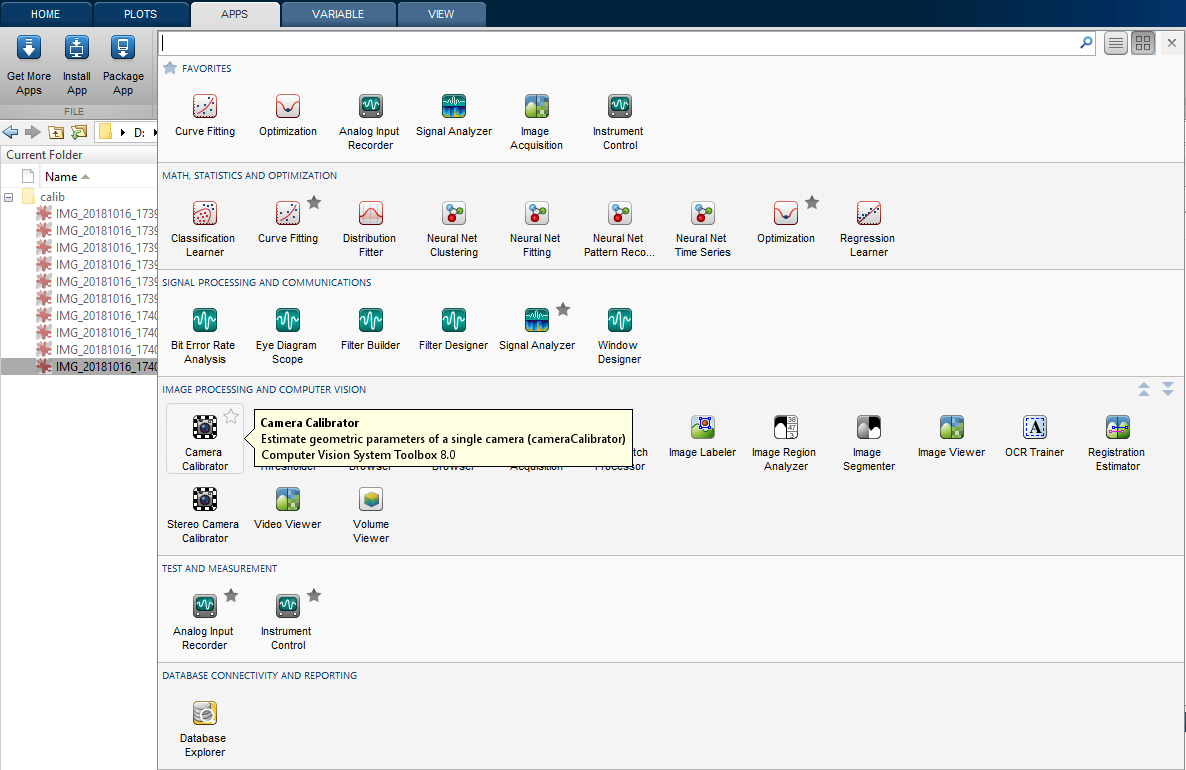
\includegraphics[width=0.7\textwidth]{calib_app.png}
\end{center}
\end{frame}

\subsection{Vonkajšie parametre}
\begin{frame}
\frametitle{Úprava obrazu}
\begin{block}{undistort}
[im, newOrigin] = undistortImage(I, cameraParams) - vráti obrázok bez skreslenia. newOrigin označuje posunutie súradníc obrazu oproti pôvodnému obrazu. V prípade, že je to [0,0] ho môžeme ignorovať.
\end{block}

\begin{block}{Úloha}
Zobrazte si neskreslený obraz pre nejaký snímok. Otestujte aj príkaz undistortImage(I, cameraParams, 'OutputView', 'full').
\end{block}

\end{frame}

\begin{frame}
\frametitle{Detekcia vzoru}
\begin{block}{detectCheckerboardPoints}
[imagePoints, boardSize] = detectCheckerboardPoints(im) - vráti pozície rohov šachovnice na obrázku a veľkosť šachovnice
\end{block}

\begin{alertblock}{detectCheckerboardPoints}
Ak sme mali posun začiatku obrazu, tak musíme posunúť aj nájdené body tj. imagePoints = imagePoints + newOrigin.
\end{alertblock}

\begin{block}{generateCheckerboardPoints}
worldPoints = generateCheckerboardPoints(boardSize, squareSize) - vráti rozloženie bodov na šachovnici, squareSize určuje šírku políčka v milimetroch.
\end{block}
\end{frame}

\begin{frame}
\frametitle{Vonkajšie parametre}

\begin{block}{extrinsics}
[R, t] = extrinsics(imagePoints, worldPoints, cameraParams) - vráti rotačnú maticu R a translačný vektor t pre dané body a parametre kamery.
\end{block}

\begin{block}{Poznámka}
Ak sme vnútorne parametre kamery zisťovali aj z obrázku kde chceme vedieť vonkajšie parametre, tak nám stačí zobrať tieto údaje zo štruktúry cameraParams.
\end{block}
\end{frame}

\begin{frame}
\frametitle{Transformácia bodov}
\begin{block}{pointsToWorld}
pointsToWorld(cameraParams, R, t, imagePoints) - vráti súradnice bodov v rovine kalibračného vzoru (v milimetroch). Na vstupe sú parametre kamery, rotačná matica, translačný vektor a matica $m \times 2$ kde v prvom stĺpci sú x-ové súradnice bodov a v druhom stĺpci sú y-ové súradnice bodov na obrázku. 
\end{block}

\begin{alertblock}{Pozor!}
Ak máme body napr. z ginput(), tak je nutné k ním opäť prirátať newOrigin, ak nieje nulový.
\end{alertblock}

\begin{block}{Úloha}
Použite ginput() a odmerajte vzdialenosť, alebo rozmery nejakého objektu pomocou tohto postupu.
\end{block}
\end{frame}

\section{Jas}
\subsection{Histogram}
\begin{frame}
\frametitle{Histogram}
\begin{block}{imhist}
imhist(I) - zobrazí histogram, v prípade že výstup zapíšeme do premennej, tak nič nevykreslí ale vráti nam vektor s histogramom.
\end{block}

\begin{block}{Úloha}
Preveďte zatisie.jpg na šedotónový obrázok. Na jeho histograme sú tri peaky. Upravte obrázok, tak aby pixely približne patriace len jednému z peakov boli úplne biele, ostatné nechajte tak.
\end{block}
\end{frame}

\subsection{Úpravy jasu}
\begin{frame}
\frametitle{Úprava jasu}
\begin{block}{Gamma korekcia}
Kontrast v obraze môžeme meniť pomocou gamma korekcie: $i_{out} = A \cdot i^{\gamma}$, kde $i$ predstavuje jas jednotlivých pixelov obrázka. Pozor jas musí byť medzi 0 a 1!
\end{block}

\begin{block}{Lineárne roztiahnutie}
Pre linárne roztiahnutie môžeme použiť nasledujúcu úpravu:
\begin{equation*}
i_{out} = \frac{i - min(I)}{max(I) - min(I)},\end{equation*}
kde i sú hodnoty jasu pre jednotlivé pixely a I predstavuje množinu jasov všetkých pixelov. Tiež chceme hodnoty jasu medzi 0 a 1.
\end{block}
\end{frame}

\begin{frame}
\frametitle{Ekvalizácia histogramu}
\begin{block}{Ekvalizácia}
Ekvalizácia histogramu je metóda, ktorá mení jas v obraze tak, aby výsledný histogram vyzeral čo najrovnomernejšie.
\end{block}

\begin{block}{histeq}
histeq(I) - vráti obrázok po ekvalizácii histogramu.
\end{block}

\begin{block}{Úloha}
Pre obrázok krajinka.png vyskúšajte rôzne metódy úpravy kontrastu. Po úpravách si zobrazte obrázky aj histogramy.
\end{block}
\end{frame}

\subsection{Prahovanie}
\begin{frame}
\frametitle{Prahovanie}
\begin{block}{imbinarize}
imbinarize(I) - vráti binarizovaný obraz s prahom určeným Otsuho metódou.
\end{block}

\begin{block}{imbinarize}
imbinarize(I, t) - vráti binarizovaný obraz s prahom t.
\end{block}

\begin{block}{Úloha}
Vyskúšajte prahovanie na obrázkoch coins.png, qr.jpg a zatisie.jpg.
\end{block}
\end{frame}

\begin{frame}
\frametitle{Adaptívne prahovanie}
\begin{block}{imbinarize}
imbinarize(I, 'adaptive') - vráti binarizovaný obraz s použitím adaptívneho prahovania.
\end{block}

\begin{block}{Úloha}
Vyskúšajte adaptívne prahovanie na obrázku coins.png a qr.jpg.
\end{block}
\end{frame}


\end{document}